% !TEX program = xelatex
\documentclass{article}

\usepackage{pgfplots}
\pgfplotsset{compat=newest}
\usepackage{tikz}


\begin{document}

% elliptic paraboloid
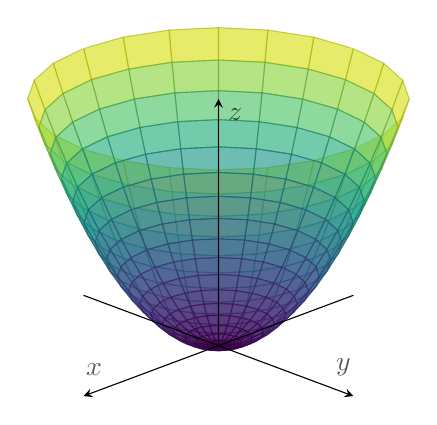
\begin{tikzpicture}
    \begin{axis}[
        axis on top,
        axis lines=center,
        set layers=default,
        xlabel={$x$}, ylabel={$y$}, zlabel={$z$},
        xtick=\empty, ytick=\empty, ztick=\empty,
        colormap/viridis,
        opacity=0.65,
        view={135}{30}
    ]

    \addplot3 [surf, draw=none,restrict z to domain=0:5,
               data cs=polar, domain=0:360, y domain=0:3] (x, y, y^2);
    \end{axis}
\end{tikzpicture}

\vspace{2em}

% cone
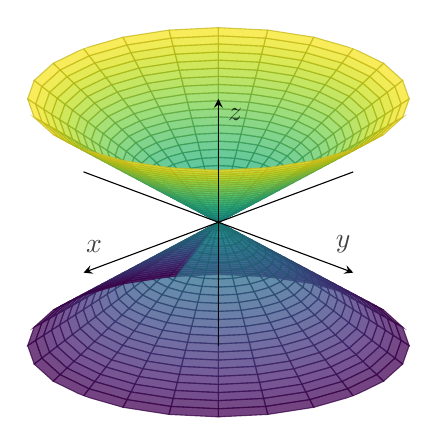
\begin{tikzpicture}
    \begin{axis}[
        axis on top,
        axis lines=center,
        set layers=default,
        xlabel={$x$}, ylabel={$y$}, zlabel={$z$},
        xtick=\empty, ytick=\empty, ztick=\empty,
        domain=0:1, y domain=0:2*pi,
        colormap/viridis,
        opacity=0.75,
        view={135}{30}
    ]

    \addplot3 [surf] ({x*cos(deg(y))}, {x*sin(deg(y))}, {x});
    \addplot3 [surf] ({x*cos(deg(y))}, {x*sin(deg(y))}, {-x});
    \end{axis}
\end{tikzpicture}

\vspace{2em}

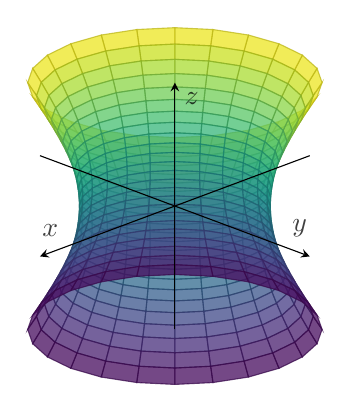
\begin{tikzpicture}
    \begin{axis}[
        axis on top,
        axis lines=center,
        set layers=default,
        xlabel={$x$}, ylabel={$y$}, zlabel={$z$},
        xtick=\empty, ytick=\empty, ztick=\empty,
        domain=0:1, y domain=0:2*pi,
        colormap/viridis,
        opacity=0.75,
        xmin=-2, xmax=2, ymin=-2, ymax=2,
        view={135}{30}
    ]

    \addplot3 [surf,domain=0:360,y domain=-1:1]
              ({cosh(y)*cos(x)}, {cosh(y)*sin(x)}, {sinh(y)});
    \end{axis}
\end{tikzpicture}


\end{document}
